\documentclass{beamer}
\usepackage[french]{babel}
\usepackage[utf8]{inputenc}
\usepackage[T1]{fontenc}
\usepackage{graphicx}
\usetheme{Madrid}
\usecolortheme{default}
\begin{document}
\title[Stage
]
{Projet Bataille Navale}

\subtitle{Présentation projet}

\author[Leroy Florent]{
  Présenté par \\
  Leroy Florent
}

\institute[]
{}

\date[20 juin 2024]
{}

\frame{\titlepage}

% Slide 2 %

%---------------------------------------------------------
\begin{frame}
  \frametitle{Présentation du jeu}
  \begin{minipage}[t]{0.48\linewidth}
    \textbf{Règle de la Bataille Navale}
    \begin{itemize}
      \item [$\bullet$] Chaque joueur dispose d'une grille de dimension $10
              \times 10$
      \item [$\bullet$] Chaque joueur pourra aussi disposer d'une grille
            supplémentaire afin de noter les tentatives d'attaques.
      \item [$\bullet$] Chaque joueur dispose de 5 bateaux de
            largeur 1 et de longueur différente :
            \begin{itemize}
              \item[$\bullet$] 1 bateau de longueur 5
              \item[$\bullet$] 1 bateau de longueur 4
              \item[$\bullet$] 2 bateaux de longueurs 3
              \item[$\bullet$] 1 bateau de longueur 2
            \end{itemize}
    \end{itemize}
  \end{minipage}\hfill
  \begin{minipage}[t]{0.48\linewidth}
    \begin{figure}[H]
      \centering
      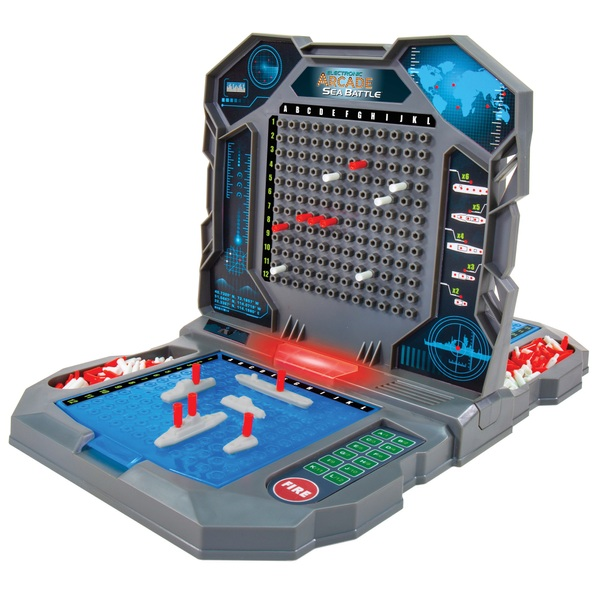
\includegraphics[width=\linewidth]{images/diapo/imageBatailleNavale.jpg}
    \end{figure}
  \end{minipage}
\end{frame}

\begin{frame}
  \frametitle{Langages utilisés}
    
  

\end{frame}

\end{document}